
%\hypertarget{aula-6}{%
%\chapter{Aula: 6}\label{aula-6}}





\hypertarget{Introdução.}{%
\chapter{Retomando às Threads.}\label{Retomando às Threads.}}




Imagine, caro leitor, que você seja dono de uma loja e que você não
tenha funcionários, como na Figura \ref{fig:Loja de único atendente}. Todas as tarefas, entre
administrar o estoque, dar baixa no caixa e atender os clientes, deve
ser feito por você. Qual estratégia você deve tomar para tornar isso
possível ?

\begin{figure}[h!]
\centering
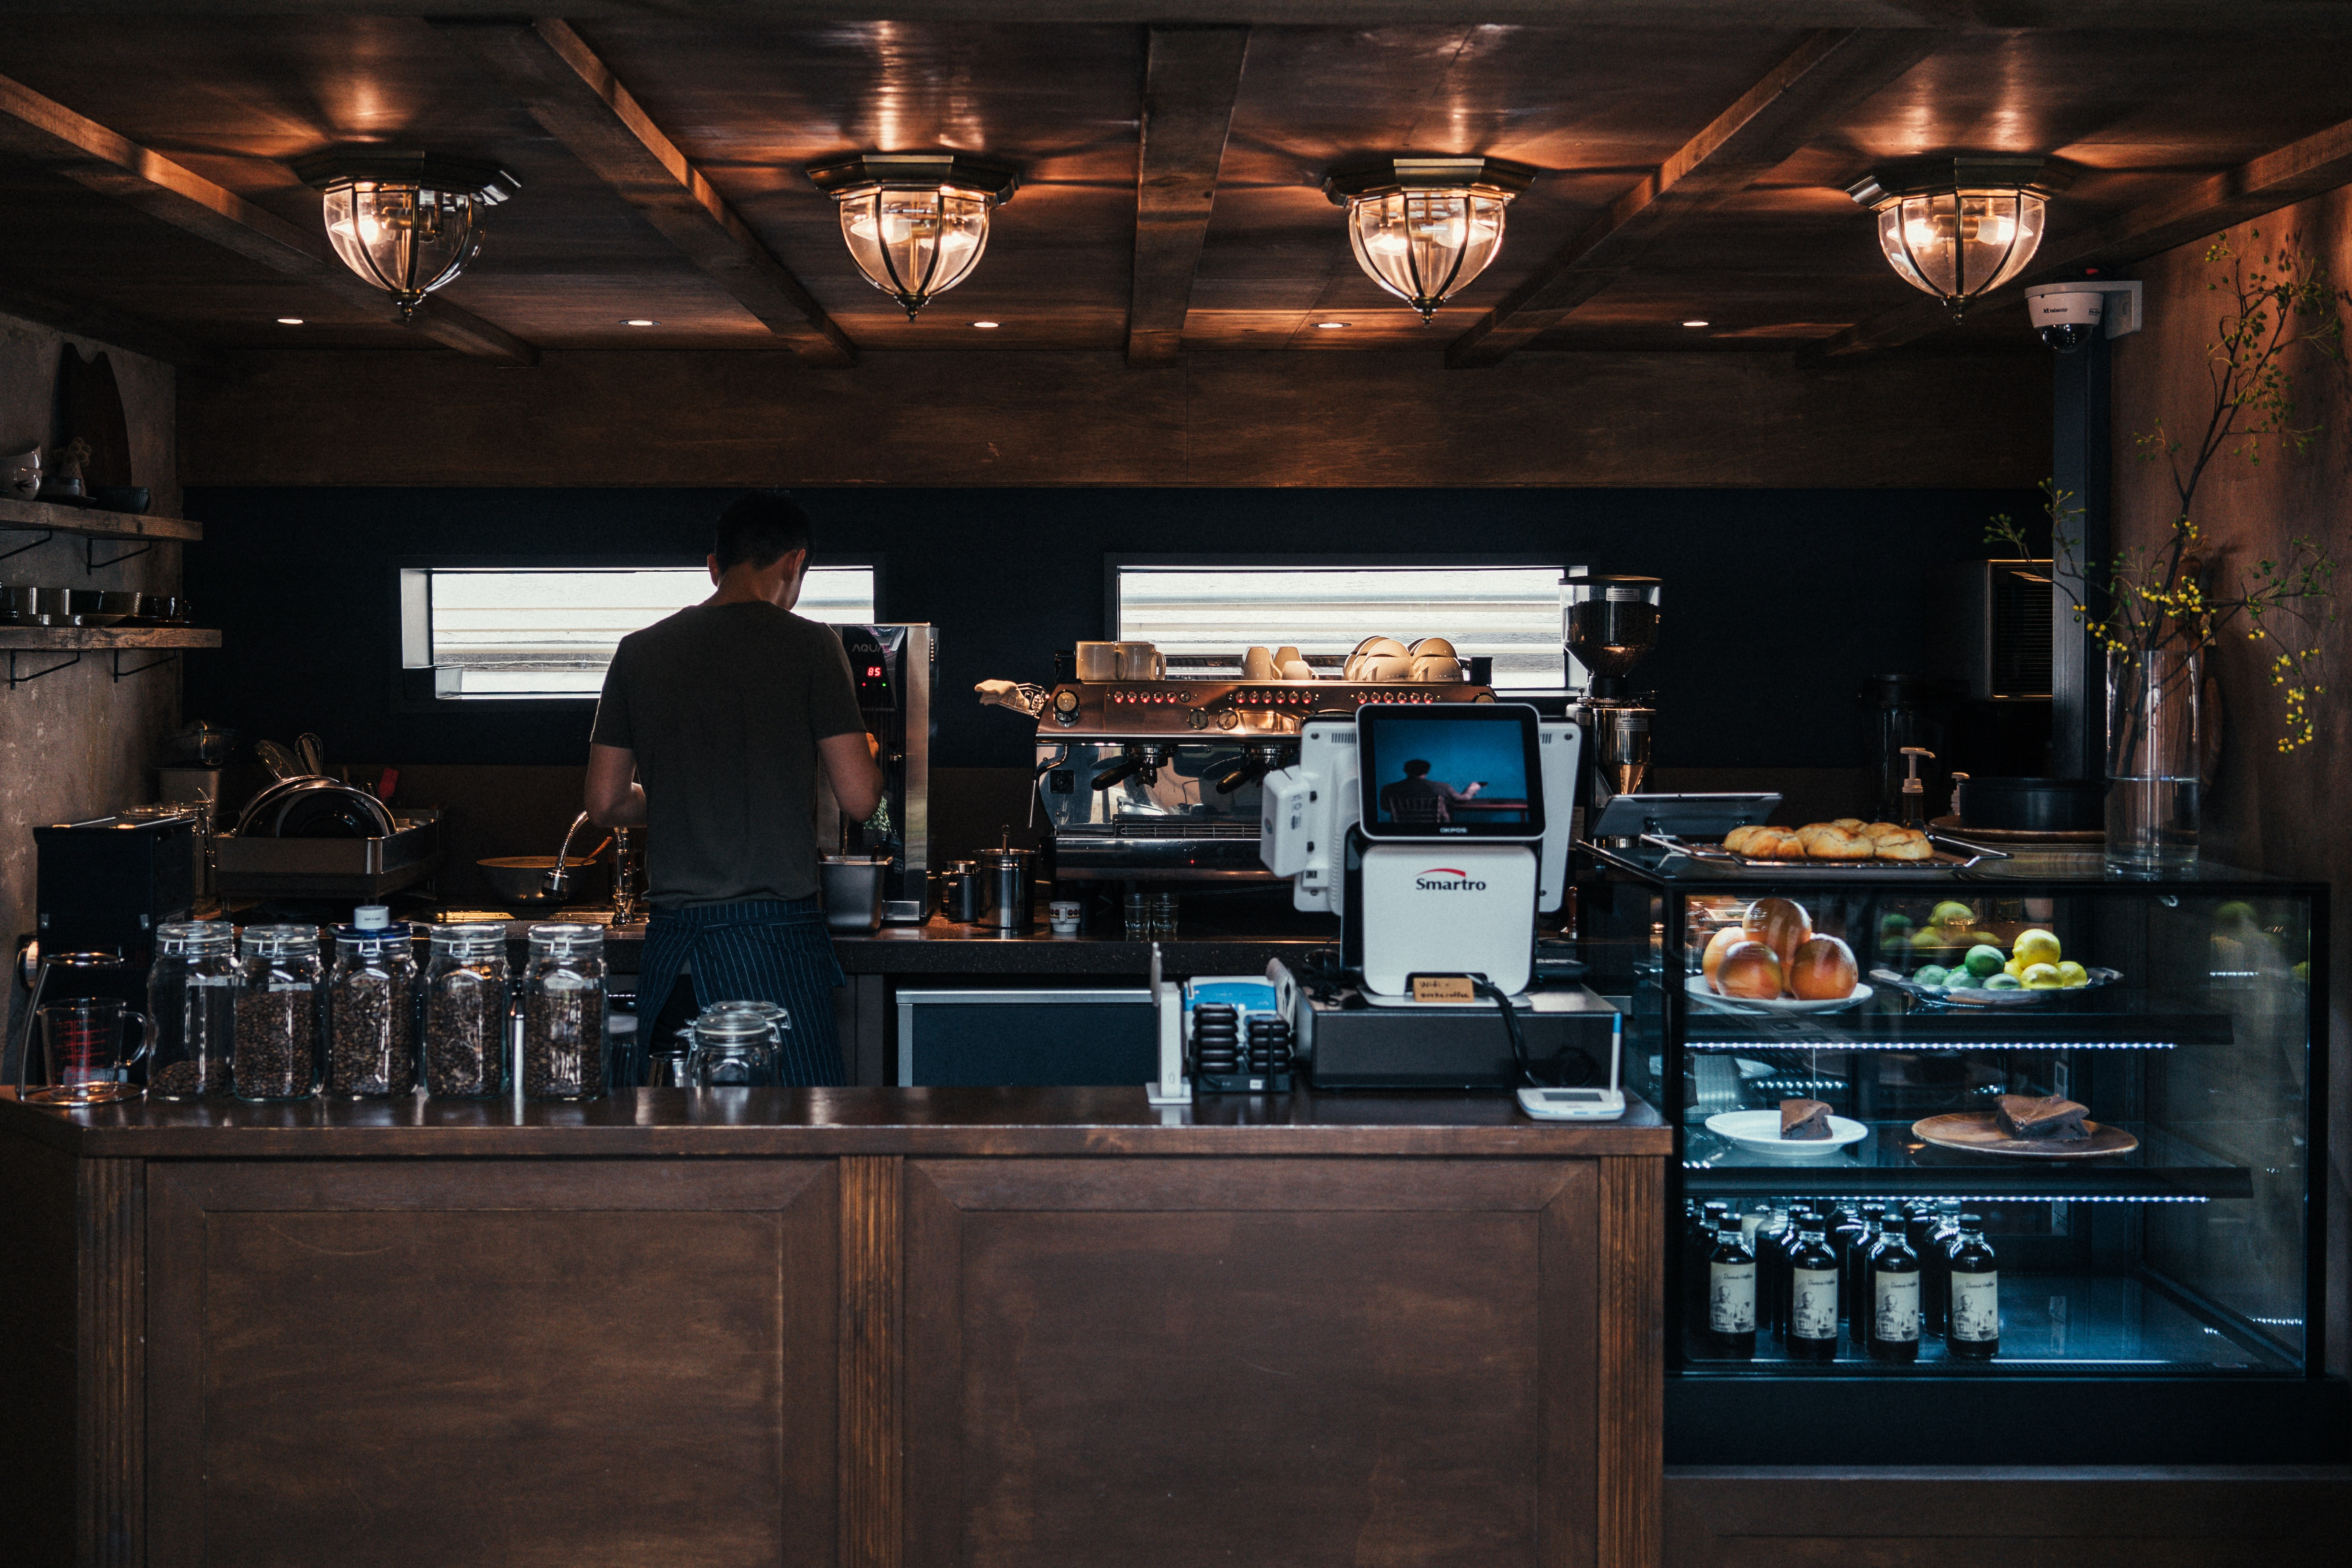
\includegraphics[keepaspectratio, width=12cm, height=9cm]{imagens/06/06 - single worker store.jpg}
\caption{Loja de único atendente   \\
Autor: rawkkim, de: unsplash.com \\}
\label{fig:Loja de único atendente}
\end{figure}

A proposta natural é a de seguir uma sequência de passos: inicialmente
deve-se chamar o primeiro cliente da fila; atendê-lo; depois administrar
o estoque; vender o produto; dar baixa no caixa; repetir o ciclo.

A vantagem é que todo o processo de venda é concluído antes de iniciar o
próximo ciclo. A desvantagem é que os novos clientes terão que esperar
bastante tempo para serem atendidos, e a fila de espera pode desanimar
possíveis compradores, como na Figura \ref{fig:Fila de espera}. É preciso perceber também que o gargalo desse processo está no atendimento ao cliente, afinal, a escolha
do cliente (ou \emph{input} do usuário do processo) não tem um momento
determinado para ocorrer. Outro problema é que um travamento (por conta
de um problema imprevisto) em uma dessas tarefas impedirá (ou atrasará)
que as próximas sejam trabalhadas.


\begin{figure}[h!]
\centering
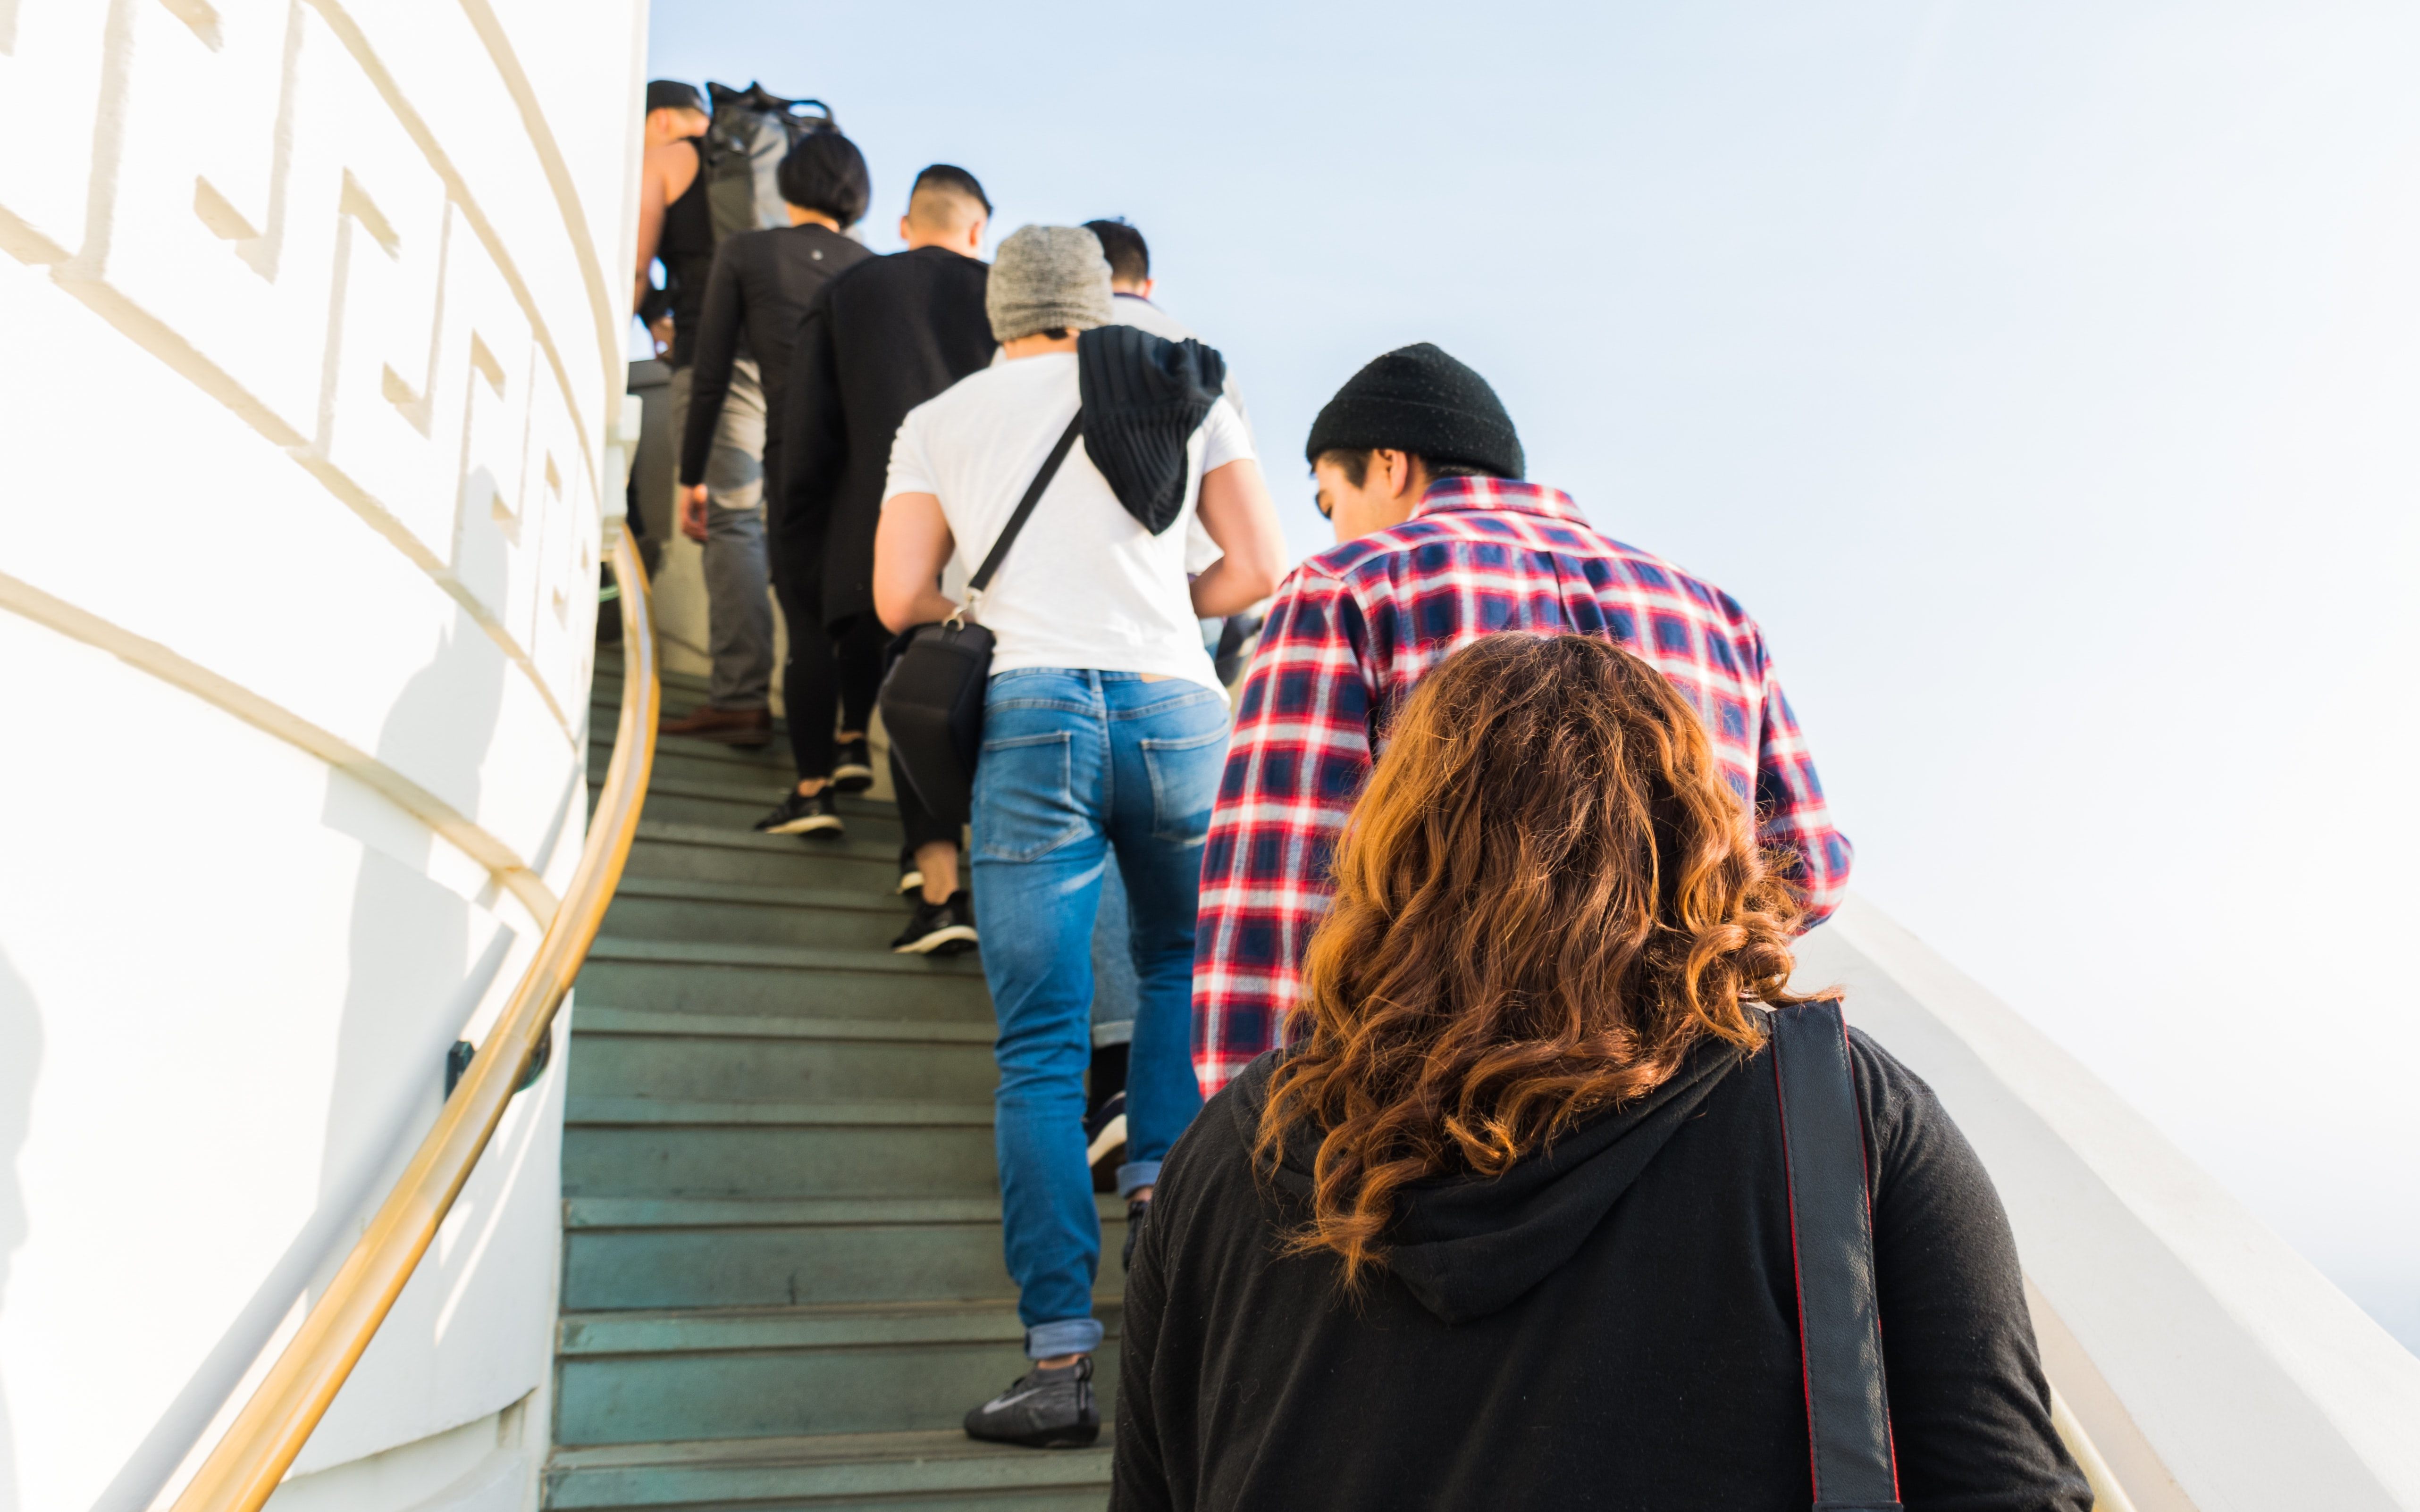
\includegraphics[keepaspectratio, width=12cm, height=9cm]{imagens/06/06 - waiting queue.jpg}
\caption{Fila de espera   \\
Autor: Levi Jones, de: unsplash.com \\}
\label{fig:Fila de espera}
\end{figure}



Para solucionar esse gargalo, poderíamos pensar em alocar, para cada
tarefa, uma parcela de tempo, digamos 10 minutos, de forma que, após
esgotado esse tempo, você terá que alterar a tarefa a ser executada,
independente se a mesma foi concluída ou não, passando para a próxima
não interdependente (\emph{non-blocking}). Assim, o leitor iniciaria o
processo chamando o primeiro da fila. Após 10 minutos, caso o
atendimento não seja concluído (por exemplo, o cliente ainda não tenha
escolhido o produto que quer), essa tarefa atualmente em trabalho será
deixada de lado (entrando no estado de espera), e a próxima tarefa não
interdependente (que no caso seria chamar o próximo da fila) deverá ser
executada. A vantagem dessa abordagem é que o tempo dentro da fila de
espera deve cair substancialmente, pois aproveita-se o tempo (no qual,
anteriormente, você ficava ocioso) de escolha (de um produto) de um
cliente, atendendo o próximo da fila.
Essa abordagem também trás desvantagens. Primeiro, você terá que
administrar (e muito bem) a prioridade e a alternância entre tarefas,
aumentando assim a complexidade do ciclo. Os clientes que fazem escolhas
rápidas podem não ficar contentes em ter que esperar que outras tarefas
relacionadas com outros compradores sejam concluídas (ou que entrem no
estado de espera) previamente, ocorrência que diminui o tempo de
resposta (responsividade) do processo. Igualmente, um número suficiente
de compradores pode tornar a responsividade tão baixa que os clientes,
simplesmente, desistirão do atendimento, derrubando a qualidade
percebida e, a loja, deixando de realizar a venda. A imposição de
padrões de qualidade (como um tempo máximo de espera por cliente), pode
resolver o problema anterior, mas criar outros, como a loja negar a
servir mais que uma quantidade específica de pessoas por período de
tempo (analogamente, ataque DDoS).
Pode-se pensar também em abrir uma segunda (ou terceira, quarta, etc)
loja ao lado, com um colaborador cada, de forma que mais clientes possam
ser atendidos. Porém, novos recursos (como caixa, material lampadas,
etc) terão que ser adquiridos, demandando tempo e dinheiro para tal.
Então, a solução mais simples (e com diversas vantagens) é a contratação
de empregados para que múltiplas tarefas possam ser desempenhadas em
paralelo, como mostrado na Figura \ref{fig:Três trabalhos em paralelo}.

\begin{figure}[h!]
\centering
\includegraphics[keepaspectratio, width=12cm, height=9cm]{imagens/06/06 - dois trabalhos em simultâneo.jpg}
\caption{Três trabalhos em paralelo   \\
Autor: Charlie Firth de: Unsplash \\}
\label{fig:Três trabalhos em paralelo}
\end{figure}


A história acima é uma analogia ao que ocorre nos sistemas
computacionais modernos, de forma que:

• O processo (em um sistema operacional) é equivalente à loja. •
Funcionários são como \emph{threads}. • Os recursos da loja (caixa,
material lampadas, etc) são como os recursos computacionais (como a
memória). • O ciclo de venda é o serviço oferecido pelo sistema
computacional. • E assim em diante.

Essa comparação é interessante pois a mesma pergunta vem à tona: devemos
criar um novo processo (abrir uma nova loja) ou, simplesmente, criar
novas \emph{threads} (contratar colaboradores) ?

O capítulo atual foi dividido em:

• Identificar os componentes de uma \emph{thread}. • Benefícios e
desafios. • \emph{Threads} e o Linux. (descrever como as \emph{threads}
são representadas no Linux e projetar uma aplicação). • Complementar

\hypertarget{identificar-os-componentes-de-uma-thread.}{%
\section{\texorpdfstring{Identificar os componentes de uma
\emph{thread}.}{Identificar os componentes de uma thread.}}\label{identificar-os-componentes-de-uma-thread.}}

A \emph{Thread} (unidade de processamento do processo) é composto pela
\emph{thread id} (seu identificador único), PC (\emph{program counter}),
valores dos registradores, memória \emph{stack}. Ela compartilha, com
outras \emph{theads} do mesmo processo, recursos como as sessões de
memória \emph{text}, \emph{data} e os arquivos abertos, como mostrado na
Figura \ref{fig:Processos com uma ou múltiplas threads}.


\begin{figure}[h!]
\centering
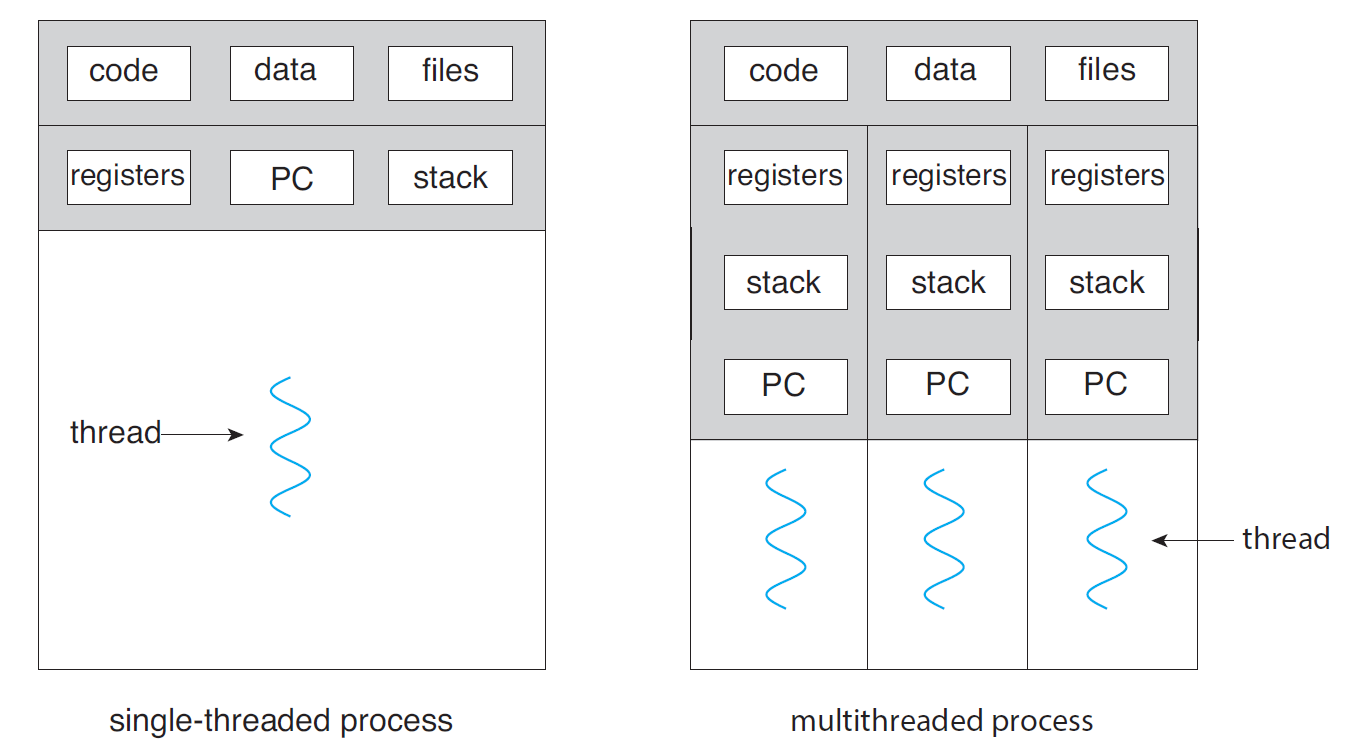
\includegraphics[keepaspectratio, width=16cm, height=15cm]{imagens/06/06 - single threaded x multi threaded.png}
\caption{Processos com uma ou múltiplas threads   \\
Imagem retirada de: Silberschatz, A. Operating System Concepts, 10th,
página 160. \\}
\label{fig:Processos com uma ou múltiplas threads}
\end{figure}



\hypertarget{benefuxedcios-e-desafios.}{%
\section{Benefícios e Desafios.}\label{benefuxedcios-e-desafios.}}

\hypertarget{benefuxedcios.}{%
\subsubsection{Benefícios.}\label{benefuxedcios.}}

Em sistemas com múltiplos núcleos de processamento, as \emph{threads}
podem trazer várias vantagens, como:

1.Responsividade: Um programa continua rodando mesmo quando uma parte
sua é bloqueada, trava ou demora para concluir. 2.Compartilhamento de
Recursos: As Threads compartilham o mesmo código e dados por padrão.
3.Economia: é mais econômico criar uma Thread do que um processo. É mais
rápido trocar o contexto da CPU (CPU context-switch) entre Threads do
que entre processos, desde que estejam em userspace. 4.Escalabilidade:
Threads podem usufruir do paralelismo, rodando em múltiplas CPU's em
simultâneo de forma assíncrona.

\hypertarget{desafios.}{%
\subsubsection{Desafios.}\label{desafios.}}

\begin{enumerate}
\def\labelenumi{\arabic{enumi}.}
\tightlist
\item
  Identificar tarefas: examinar a aplicação e separá-la em diferentes
  tarefas que possam ser executadas em paralelo.
\item
  Balancear: a carga de trabalho deve ser distribuída entre as tarefas
  (idealmente, as tarefas teriam a mesma carga).
\item
  Divisão de dados: os dados devem sem divididos para rodar em núcleos
  de processamento separados (para evirar a \emph{race condition}).
\item
  Dependência de dados: os programadores devem garantir que as tarefas
  estejam sincronizadas quando uma \emph{thread} depende dos dados de
  outra.
\item
  Teste: é mais difícil testar e replicar casos de erro em sistemas com
  múltiplas \emph{threads} em comparação com as de \emph{thread} única.
\end{enumerate}

\hypertarget{modelos-de-multithread}{%
\section{Modelos de multithread}\label{modelos-de-multithread}}

Há dois tipos diferentes de \emph{threads}, aquelas que estão no nível
de usuário, sendo gerenciadas sem ajuda do \emph{kernel}, e aquelas que
estão no nível do \emph{kernel}, que são gerenciadas diretamente pelo
sistema operacional. Assim, os modelos de \emph{multithread} definem o
relacionamento desses dois tipos de \emph{threads}.


\begin{enumerate}
\def\labelenumi{\arabic{enumi}.}

\item
  \emph{Many-to-one} (Figura \ref{fig:Modelo Many-to-One}): nesse modelo, várias \emph{threads} de nível do
  usuário são mapeadas para uma única \emph{thread} de \emph{kernel}.
\item
  \emph{One-to-one} (Figura \ref{fig:Modelo One-to-One}): cada \emph{thread} de usuário tem, mapeada, uma
  \emph{thread} de \emph{kernel}.
\item
  \emph{Many-to-many} (Figura \ref{fig:Modelo Many-to-Many}): várias \emph{threads} de usuário são
  multiplexadas entre as diferentes \emph{threads} de kernel.
\item
  \emph{Two-level} (Figura \ref{fig:Modelo two-level}): esse modelo une o \emph{one-to-one} com o
  \emph{many-to-many}.
\end{enumerate}



\begin{figure}[h!]
\centering
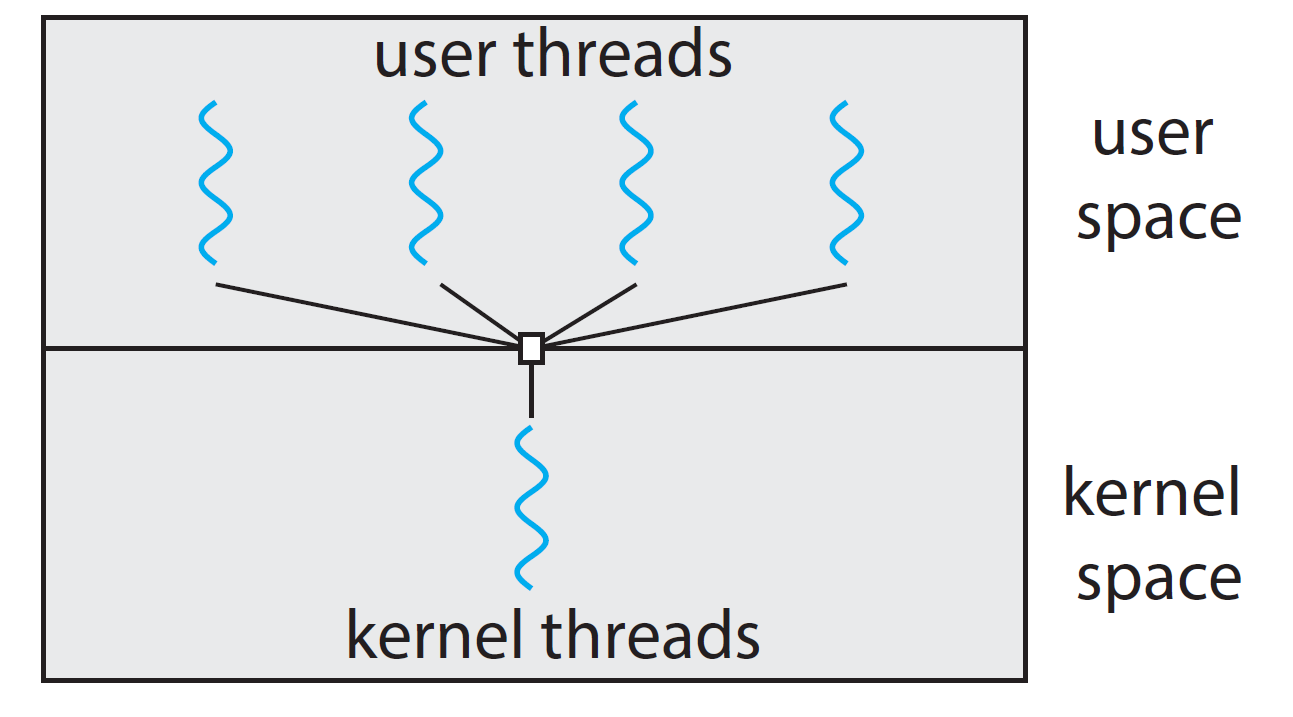
\includegraphics[keepaspectratio, width=12cm, height=9cm]{imagens/06/06 - many-to-one.png}
\caption{Modelo Many-to-One   \\
Imagem retirada de: Silberschatz, A. Operating System Concepts, 10th,
página 166. \\}
\label{fig:Modelo Many-to-One}
\end{figure}

\begin{figure}[h!]
\centering
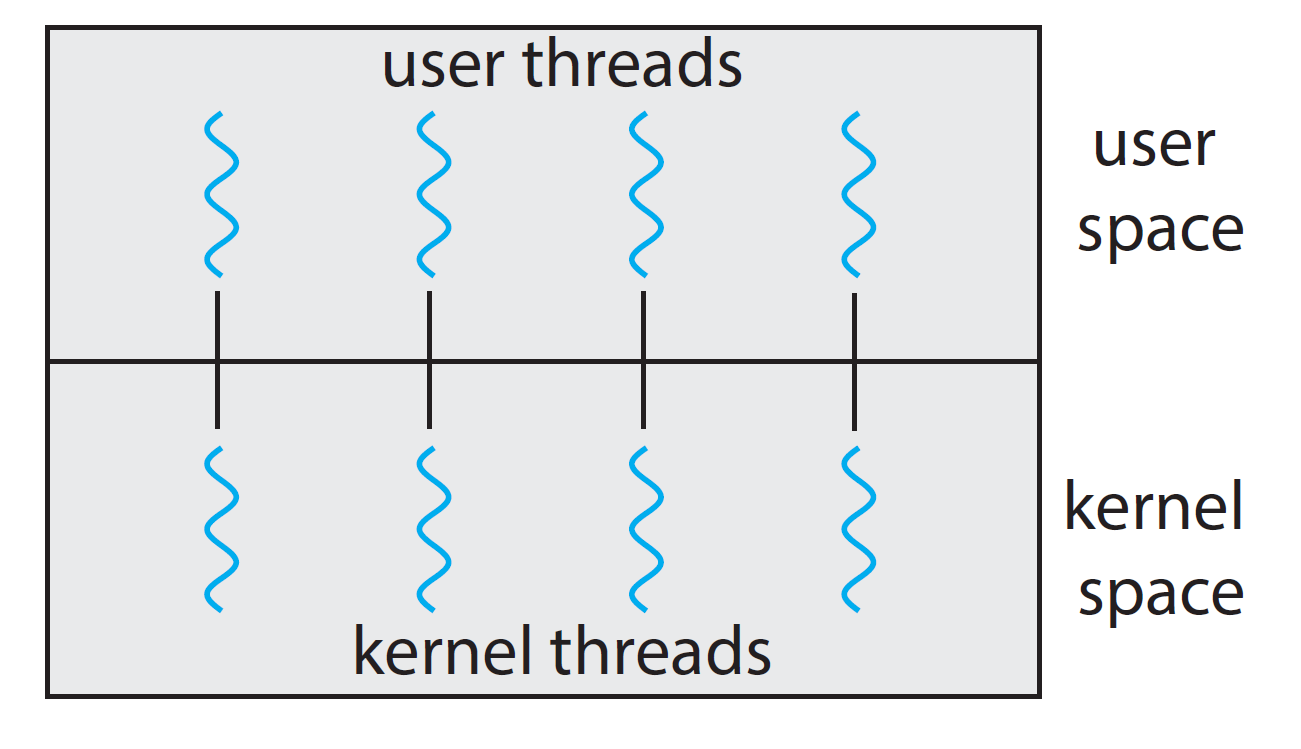
\includegraphics[keepaspectratio, width=12cm, height=9cm]{imagens/06/06 - one-to-one.png}
\caption{Modelo One-to-One   \\
Imagem retirada de: Silberschatz, A. Operating System Concepts, 10th,
página 167. \\}
\label{fig:Modelo One-to-One}
\end{figure}

\begin{figure}[h!]
\centering
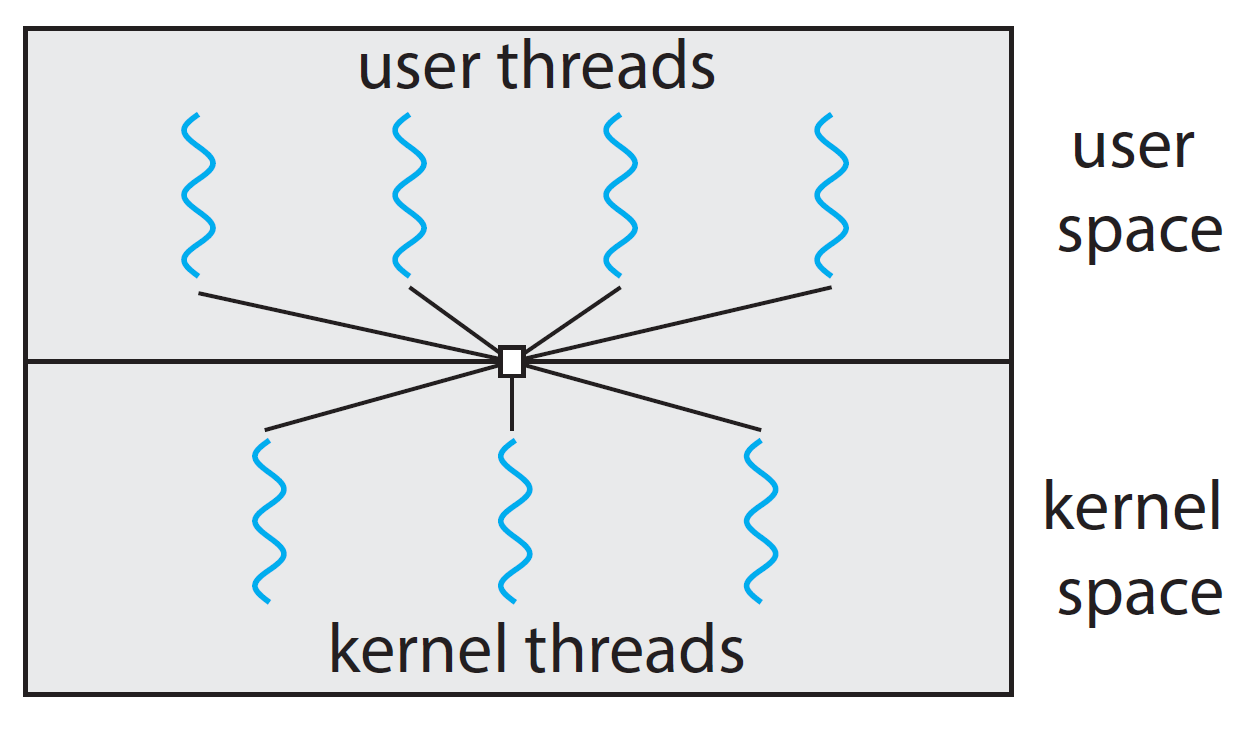
\includegraphics[keepaspectratio, width=12cm, height=9cm]{imagens/06/06 - many-to-many.png}
\caption{Modelo Many-to-Many  \\
Imagem retirada de: Silberschatz, A. Operating System Concepts, 10th,
página 167. \\}
\label{fig:Modelo Many-to-Many}
\end{figure}


\begin{figure}[h!]
\centering
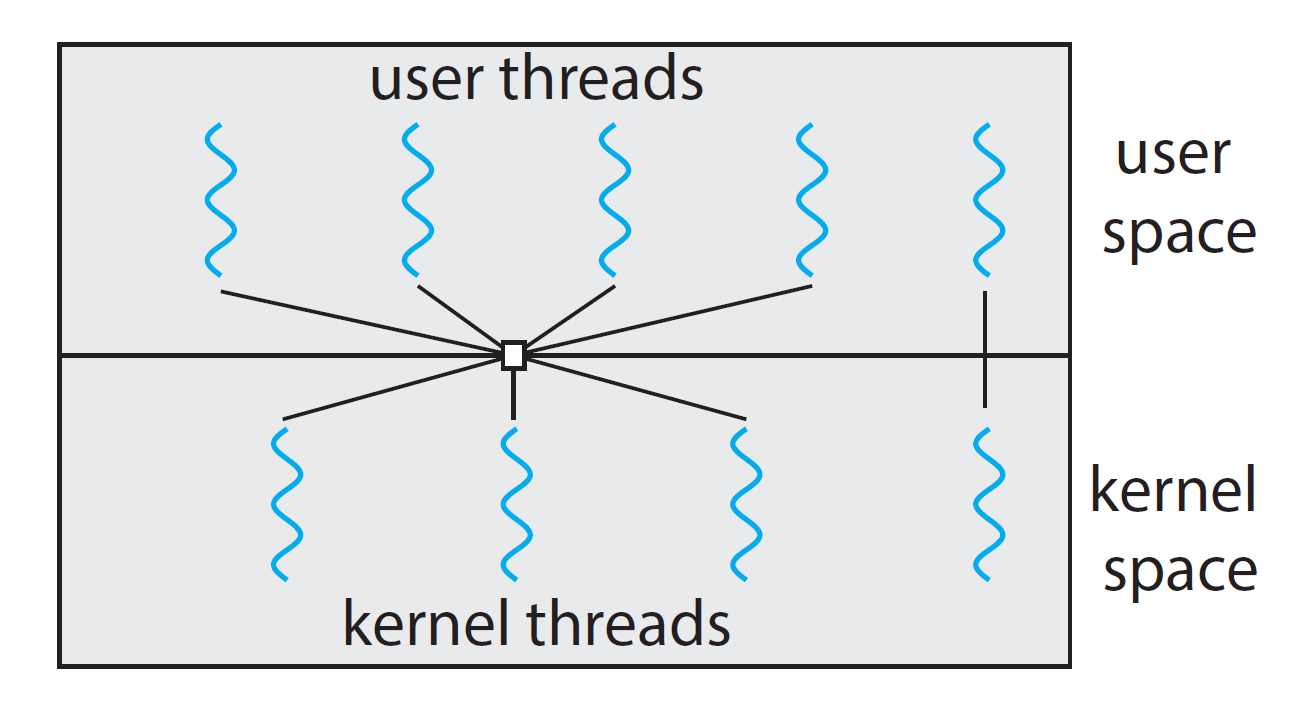
\includegraphics[keepaspectratio, width=12cm, height=9cm]{imagens/06/06 - two-level.png}
\caption{Modelo two-level  \\
Imagem retirada de: Silberschatz, A. Operating System Concepts, 10th,
página 168. \\}
\label{fig:Modelo two-level}
\end{figure}


\hypertarget{threads-e-o-linux}{%
\section{Threads e o Linux}\label{threads-e-o-linux}}

\hypertarget{biblioteca-pthread}{%
\subsection{\texorpdfstring{Biblioteca
\texttt{pthread}}{Biblioteca pthread}}\label{biblioteca-pthread}}

O Linux utiliza a biblioteca POSIX \emph{threads}, nomeada, em
\texttt{C}, de \texttt{pthread}.

O exemplo a seguir foi retirado de: Silberschatz, A. Operating System
Concepts, 10th, página 170.*


\begin{minted}[mathescape, linenos]{c}

    #include <pthread.h>
    #include <stdio.h>
    #include <stdlib.h>
    
    int sum; /* this data is shared by the thread(s) */
    void *runner(void *param); /* threads call this function */
    
    int main(int argc, char *argv[])
    {
        pthread_t tid; /* the thread identifier */
        pthread_attr_t attr; /* set of thread attributes */
        /* set the default attributes of the thread */
        pthread_attr_init(&attr);
        /* create the thread */
        pthread_create(&tid, &attr, runner, argv[1]);
        /* wait for the thread to exit */
        pthread_join(tid,NULL);
        printf("sum = %d∖n",sum);
    }
    
    /* The thread will execute in this function */
    void *runner(void *param)
    {
        int i, upper = atoi(param);
        sum = 0;
        for (i = 1; i <= upper; i++)
        sum += i;
        pthread exit(0);
    }
    
\end{minted}


\hypertarget{semuxe1foros}{%
\subsection{Semáforos}\label{semuxe1foros}}

A execução em paralelo de várias \emph{threads} (de dados
compartilhados) pode gerar uma \emph{race condition} (conceito debatido
em capítulos anteriores) por poder alterar, com dados desatualizados, o
mesmo valor. Considere:

\begin{minted}[mathescape, linenos]{c}

    int a = 5;
    a = a - 1;
    
\end{minted}



A \emph{thread} ``A'' e ``B'', executando em paralelo, podem gerar o
resultado final de 4, e não de 3, como esperado, Pois:

\begin{enumerate}
\def\labelenumi{\arabic{enumi}.}
\tightlist
\item
  \emph{Thread} ``A'' coleta o valor de \texttt{a} (5).
\item
  \emph{Thread} ``B'' coleta o valor de \texttt{a} (5).
\item
  \emph{Thread} ``B'' calcula \texttt{a\ -\ 1} (4).
\item
  \emph{Thread} ``A'' calcula \texttt{a\ -\ 1} (4).
\item
  \emph{Thread} ``A'' ajusta o valor de \texttt{a} (4).
\item
  \emph{Thread} ``B'' ajusta o valor de \texttt{a} (4).
\end{enumerate}

Esse caso fica visível no exemplo a seguir:

Exemplo retirada de: Griffiths, David; Griffiths, Dawn; Head First C,
página 510.

\begin{minted}[mathescape, linenos]{c}

    #include <stdio.h>
    #include <stdlib.h>
    #include <string.h>
    #include <unistd.h>
    #include <errno.h>
    #include <pthread.h>
    
    int beers = 2000000;
    void* drink_lots(void *a)
    {
    int i;
    for (i = 0; i < 100000; i++) {
    beers = beers - 1;
    }
    return NULL;
    }
    int main()
    {
    pthread_t threads[20];
    int t;
    printf("%i bottles of beer on the wall\n%i bottles of beer\n", beers, beers);
    for (t = 0; t < 20; t++) {
    ( , NULL, , NULL);
    }
    void* result;
    for (t = 0; t < 20; t++) {
    pthread_create(threads[t], &result);
    }
    printf("There are now %i bottles of beer on the wall\n", beers);
    return 0;
    }
    pthread_join
    &threads[t]
    drink_lots
    
\end{minted}


no qual, o trecho abaixo (região crítica) necessita ser protegido pelo
acesso múltiplo, como explicado anteriormente.

\begin{minted}[mathescape, linenos]{c}

    for (i = 0; i < 100000; i++) {
        beers = beers - 1;
    }
    
\end{minted}



Sem essa proteção, os resultados serão:

Resultados retirados de: Griffiths, David; Griffiths, Dawn; Head First
C, página 511.

\begin{lstlisting}[language=bash]
    > ./beer 
    2000000 bottles of beer on the wall 
    2000000 bottles of beer 
    There are now 0 bottles of beer on the wall 
    > ./beer 
    2000000 bottles of beer on the wall 
    2000000 bottles of beer 
    There are now 883988 bottles of beer on the wall 
    > ./beer 2000000 bottles of beer on the wall 
    2000000 bottles of beer 
    There are now 945170 bottles of beer on the wall ```
\end{lstlisting}



Perceba que, sem proteção, os resultados não são consistentes.

Para que essas duas \emph{threads} trabalhem de forma síncrona, é
necessário que haja um semáforo (mesmo conceito de controle de tráfego
de carros), para o controle de acesso, como mostrado na Figura \ref{fig:Semáforo para controle de acesso.}. Os
semáforos que previnem que as \emph{threads} não se choquem são chamadas
de \texttt{mutex} (\emph{mutually exclusive}, só permite uma única
\emph{thread} na região crítica) e também de \texttt{locks}.


\begin{figure}[h!]
\centering
\includegraphics[keepaspectratio, width=12cm, height=9cm]{imagens/06/06 - semáforo.png}
\caption{Semáforo para controle de acesso.  \\
Imagem retirada de: Griffiths, David; Griffiths, Dawn; Head First C,
página 513. \\}
\label{fig:Semáforo para controle de acesso.}
\end{figure}



Existem, então, duas soluções para o trecho de código anterior, cada
qual gerará resultados de saída, desempenho e sincronicidade diferentes.

Solução A.


\begin{minted}[mathescape, linenos]{c}

    pthread_mutex_t beers_lock = PTHREAD_MUTEX_INITIALIZER;
    
    void* drink_lots(void *a)
    {
        int i;
        pthread_mutex_lock(&beers_lock);
        
        for (i = 0; i < 100000; i++) {
            beers = beers - 1;
        }
        
        pthread_mutex_unlock(&beers_lock);
        printf("beers = %i\n", beers);
        return NULL;
    }
    
\end{minted}





Solução B.

\begin{minted}[mathescape, linenos]{c}

    pthread_mutex_t beers_lock = PTHREAD_MUTEX_INITIALIZER;
    
    void* drink_lots(void *a)
    {
        int i;
        
        for (i = 0; i < 100000; i++) {
            pthread_mutex_lock(&beers_lock);
            beers = beers - 1;
            pthread_mutex_unlock(&beers_lock);
        }
        
        printf("beers = %i\n", beers);
        return NULL;
    }
    
\end{minted}



Resultados retirados de: Griffiths, David; Griffiths, Dawn; Head First
C, página 517.

Resultado Versão A.

\begin{lstlisting}[language=bash]
    > ./beer
    2000000 bottles of beer on the wall
    2000000 bottles of beer
    beers = 1900000
    beers = 1800000
    beers = 1700000
    beers = 1600000
    beers = 1500000
    beers = 1400000
    beers = 1300000
    beers = 1200000
    beers = 1100000
    beers = 1000000
    beers = 900000
    beers = 800000
    beers = 700000
    beers = 600000
    beers = 500000
    beers = 400000
    beers = 300000
    beers = 200000
    beers = 100000
    beers = 0
    There are now 0 bottles of beer on the wall
    >
\end{lstlisting}



Resultado Versão B.

\begin{lstlisting}[language=bash]
    > ./beer_fixed_strategy_2
    2000000 bottles of beer on the wall
    2000000 bottles of beer
    beers = 63082
    beers = 123
    beers = 104
    beers = 102
    beers = 96
    beers = 75
    beers = 67
    beers = 66
    beers = 65
    beers = 62
    beers = 58
    beers = 56
    beers = 51
    beers = 41
    beers = 36
    beers = 30
    beers = 28
    beers = 15
    beers = 14
    beers = 0
    There are now 0 bottles of beer on the wall
>

\end{lstlisting}



\hypertarget{complementar-2}{%
\section{Complementar}\label{complementar-2}}

\hypertarget{tuxe9cnicas-de-paralelismo.}{%
\subsection{Técnicas de
paralelismo.}\label{tuxe9cnicas-de-paralelismo.}}

Fundamentalmente, existem dois tipos diferentes de paralelismo, o
paralelismo de tarefas (\emph{task parallelism}), que consiste em
dividir múltiplas tarefas compartilhando os dados necessários, e o
paralelismo de dados (\emph{data parallelism}), o qual há uma
distribuição dos dados sobre as tarefas.


\begin{figure}[H]
\centering
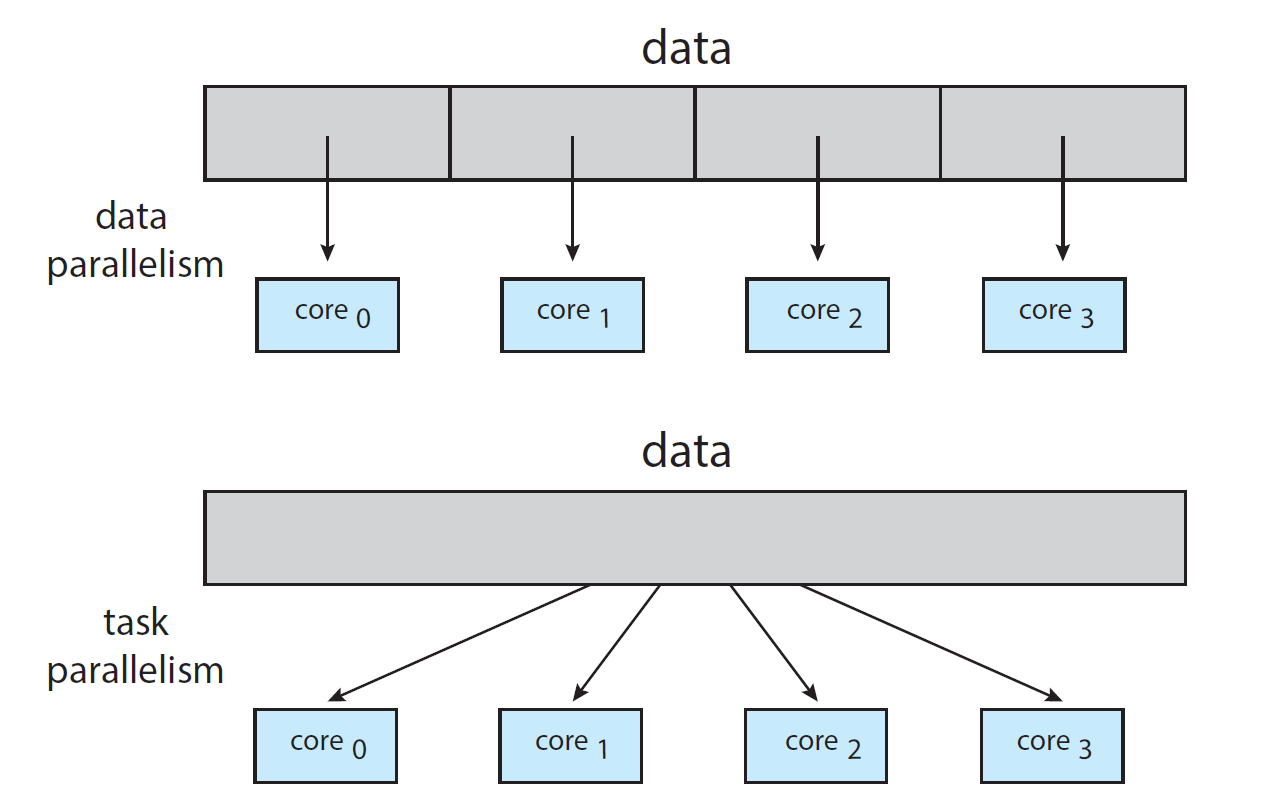
\includegraphics[keepaspectratio, width=12cm, height=9cm]{imagens/06/06 - data and task parallelism.png}
\caption{Processos com uma ou múltiplas threads  \\
Silberschatz, A. Operating System Concepts, 10th, página 170. \\
}
\label{fig:Processos com uma ou múltiplas threads}
\end{figure}
